\documentclass[9pt,t]{beamer}
% note that full page width is 12.8 cm and height is 9.6 cm

\mode<presentation>
{
  \usepackage[headline,footline]{beamerthemelectures}

}

% load packages
\usepackage[english]{babel}
\usepackage{graphicx}
\usepackage{multimedia}
%\usepackage[T1]{fontenc}
\usepackage{lmodern}
\usepackage{amsmath,amssymb}
\usepackage{pgf,booktabs,verbatim}
\usepackage{pgfarrows,pgfnodes}
\usepackage[absolute,overlay]{textpos}
\setlength{\TPHorizModule}{\paperwidth}
\setlength{\TPVertModule}{\paperheight}
\usepackage{tikz}

\setbeamertemplate{frametitle}{
\begin{centering}
\insertframetitle
\par
\end{centering}
} 

% create command to add nice looking citation
\newcommand{\reference}[1]{\flushright \vspace{-0.3cm} {\tiny #1}} 


\title{Solutions to Modeling Exercise \#6\\ The carbon cycle}

\begin{document}

\section{}

%%%
\frame{
    \frametitle{\vspace{1cm}\huge The carbon cycle}
   
}

\frame{
\frametitle{1. Turn off fossil fuel and land use change switches}
\begin{figure}
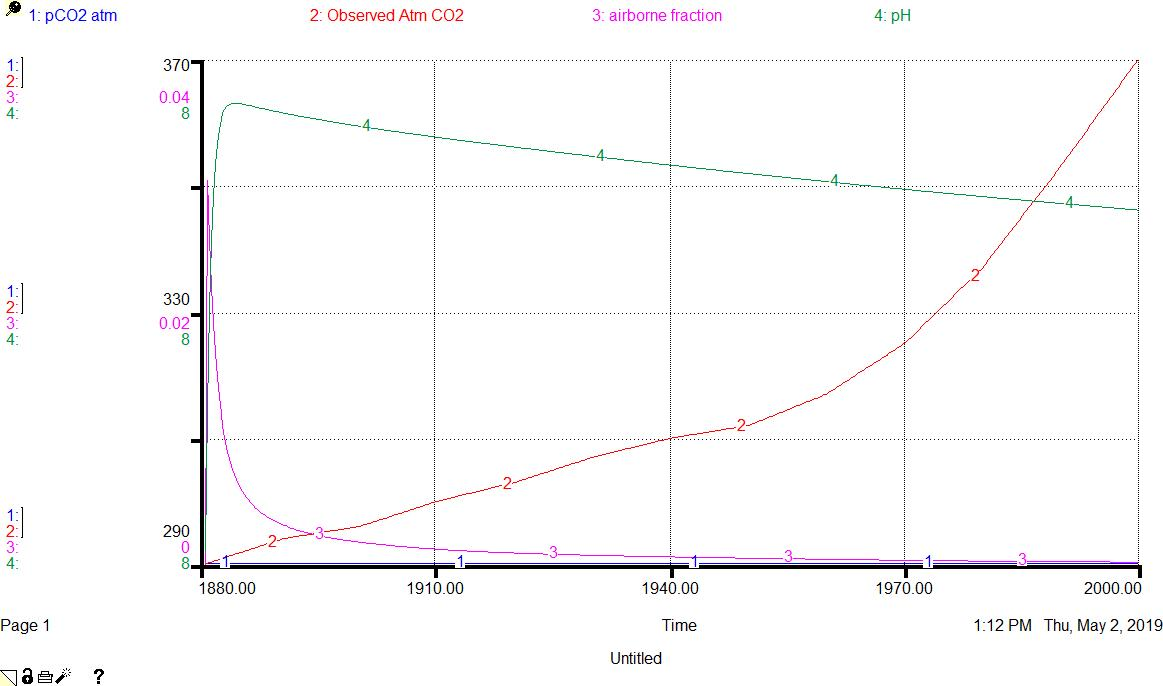
\includegraphics[width=0.9\textwidth]{./p1-a.jpg}
\end{figure}
\begin{itemize}
\item System is in a steady state.
\end{itemize}
}

\frame{
\frametitle{1. Turn switches on}
\begin{figure}
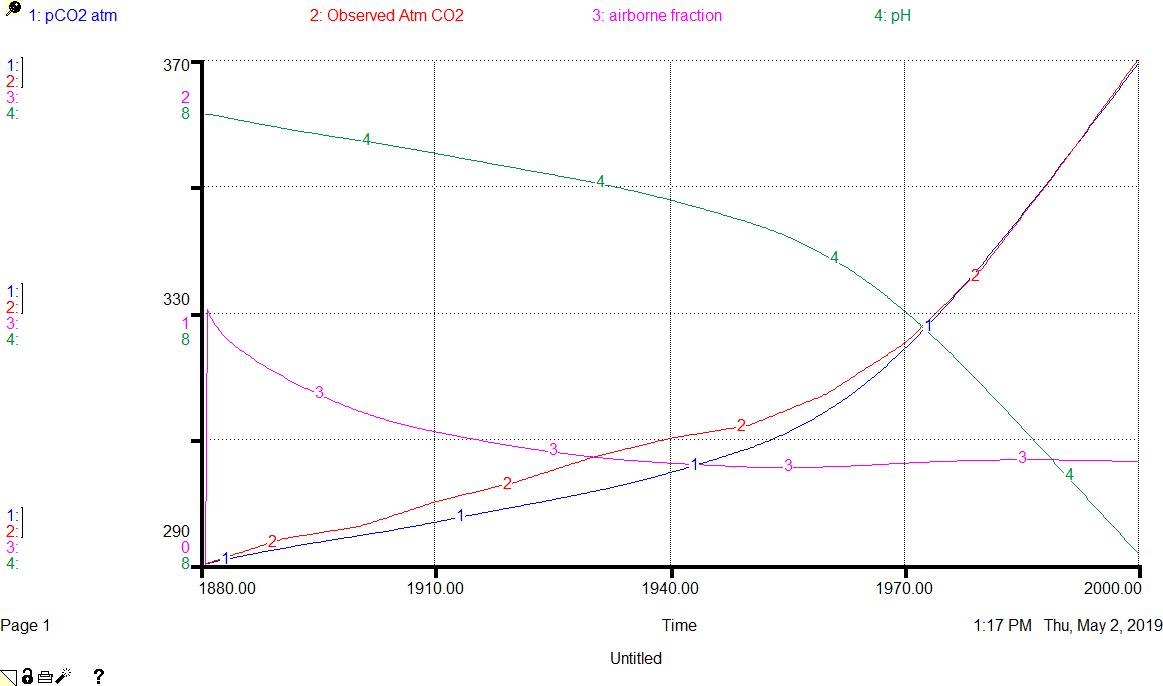
\includegraphics[width=0.9\textwidth]{./p1-b.jpg}
\end{figure}
\begin{itemize}
\item Observed and modeled CO$_2$ are about the same
\item Similar starting and ending values; slightly different pathways
\end{itemize}
}

\frame{
\frametitle{2.1. Turn off ocean mixing}
\begin{figure}
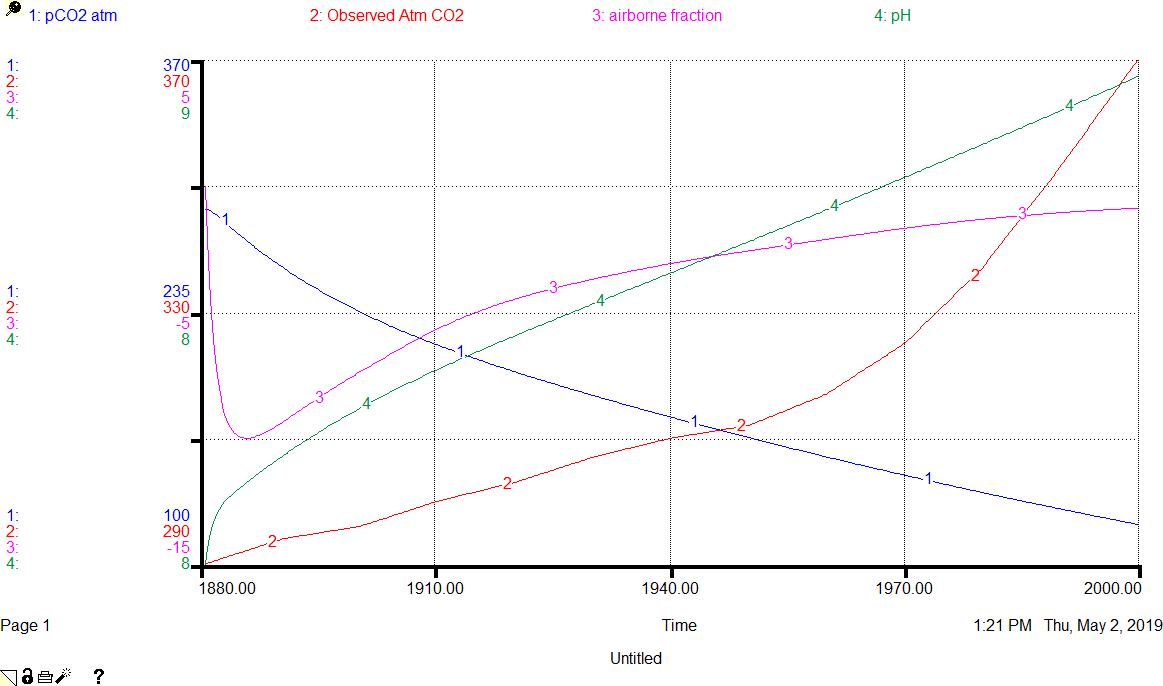
\includegraphics[width=0.9\textwidth]{./p2-1.jpg}
\end{figure}
\begin{itemize}
\item Modeled CO$_2$ dropped by $\sim$200 ppm
\end{itemize}
}

\frame{
\frametitle{2.2. Increase biological mixing with time}
\begin{figure}
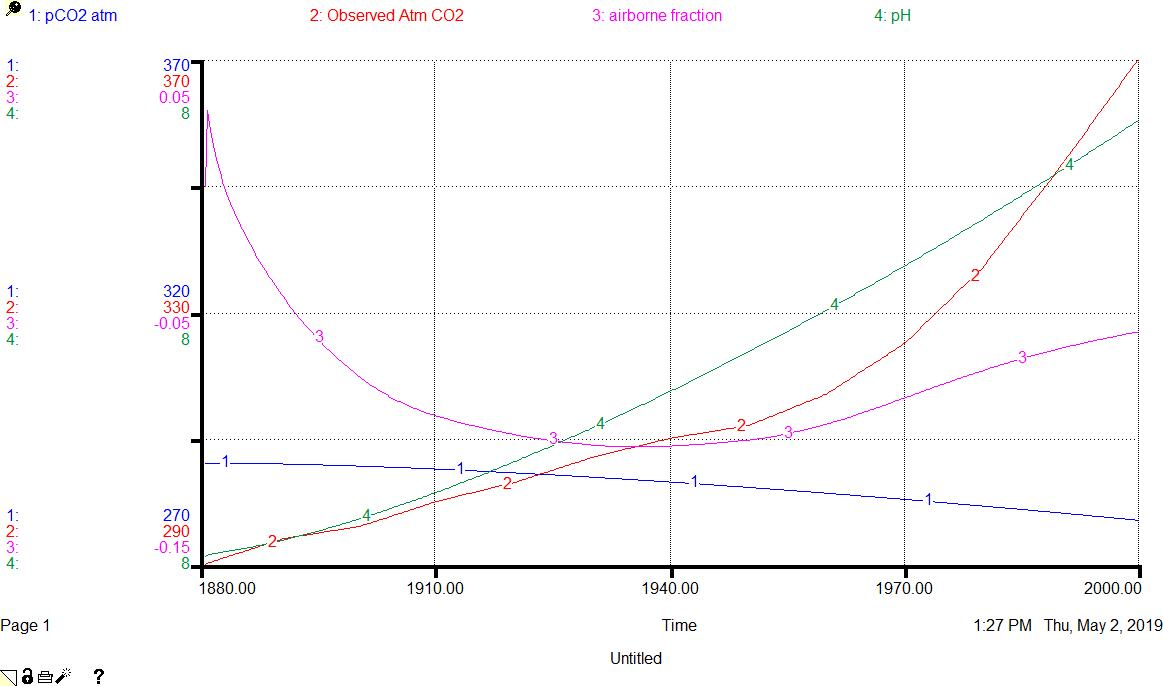
\includegraphics[width=0.9\textwidth]{./p2-2.jpg}
\end{figure}
\begin{itemize}
\item CO$_2$ decreases by 200 ppm over 120 years
\end{itemize}
}

\frame{
\frametitle{2.2. Increase biological mixing with time}
\begin{figure}
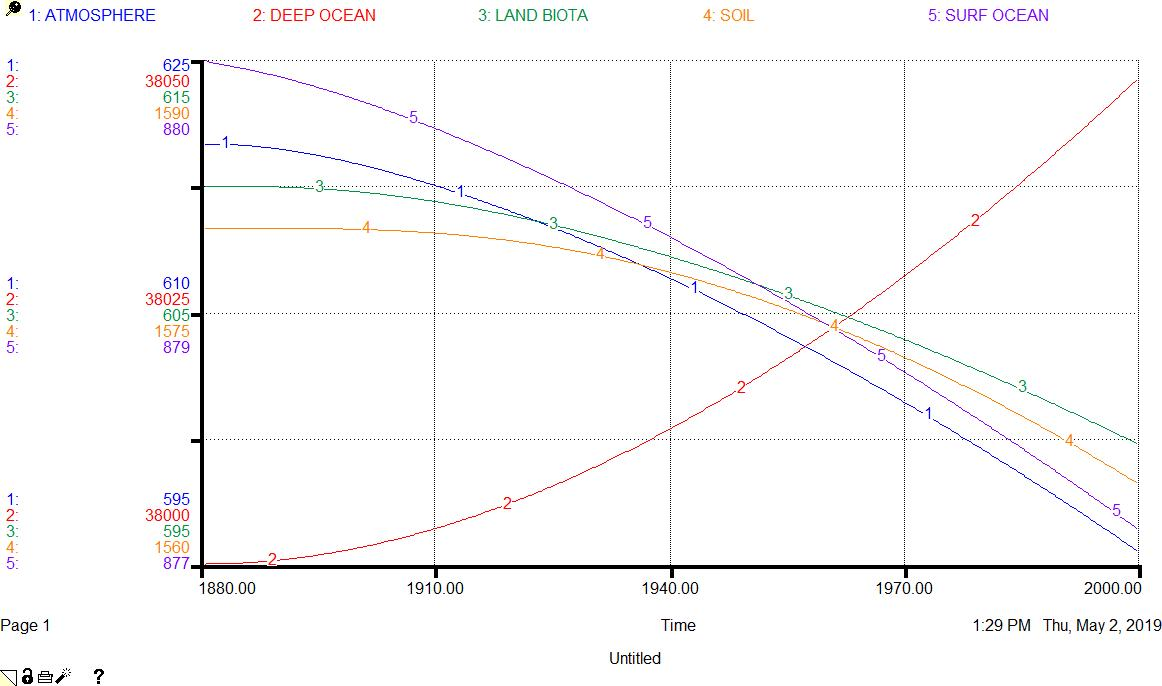
\includegraphics[width=0.9\textwidth]{./p2-2b.jpg}
\end{figure}
\begin{itemize}
\item All reservoirs except deep ocean gradually decrease with time
\end{itemize}
}

\frame{
\frametitle{2.3. Volcanic eruption (increase by 0.2 for 2 years)}
\begin{figure}
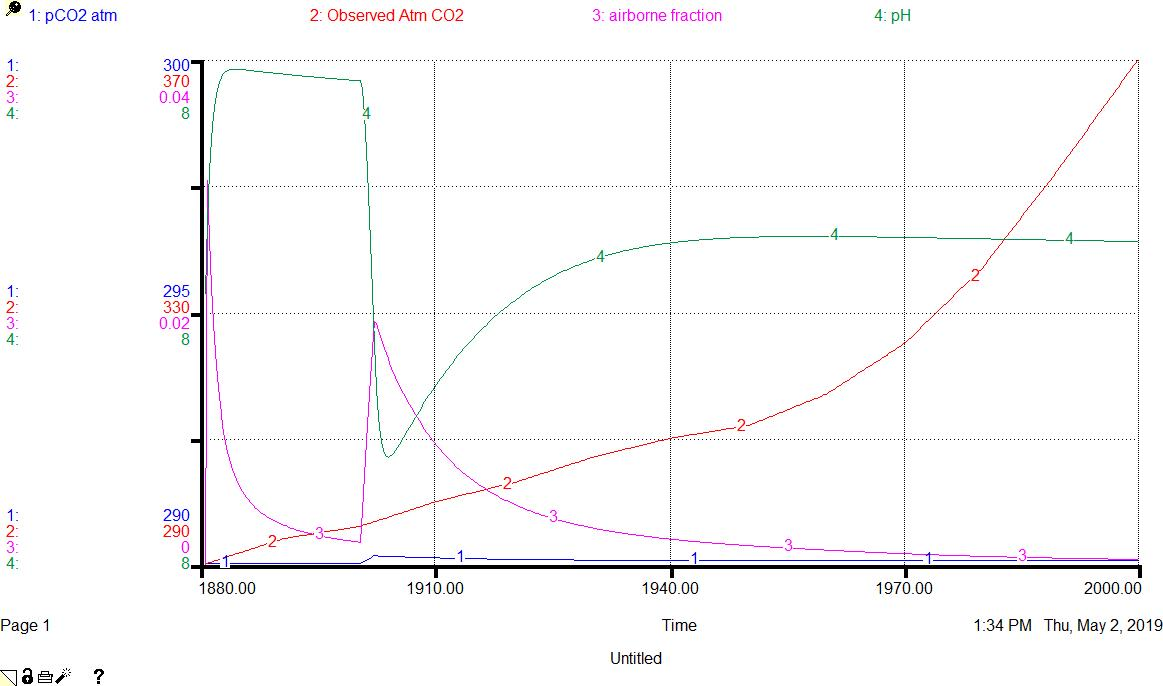
\includegraphics[width=0.9\textwidth]{./p2-3a.jpg}
\end{figure}
\begin{itemize}
\item Small change in atmospheric CO$_2$ concentrations
\item e-folding time of $\sim$10 a
\end{itemize}
}

\frame{
\frametitle{2.3. Volcanic eruption (increase by 0.2 for 2 years)}
\begin{figure}
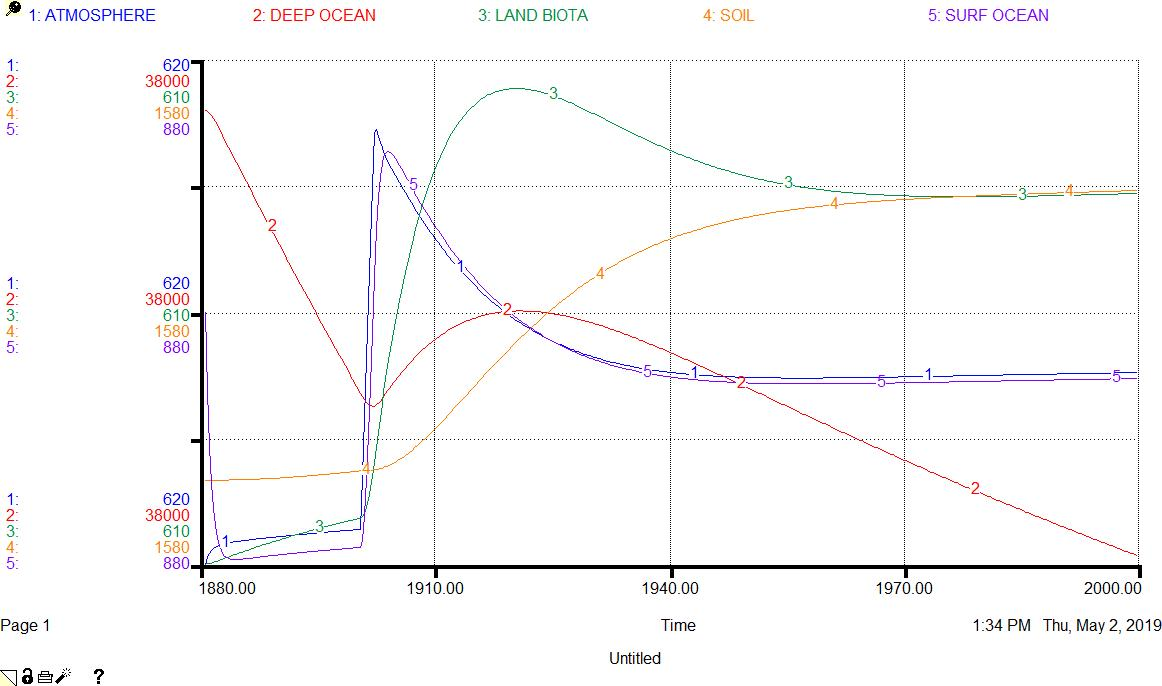
\includegraphics[width=0.9\textwidth]{./p2-3b.jpg}
\end{figure}
\begin{itemize}
\item Surface ocean absorbed much of the CO$_2$
\end{itemize}
}

\frame{
\frametitle{3.1. Business as usual}
\begin{figure}
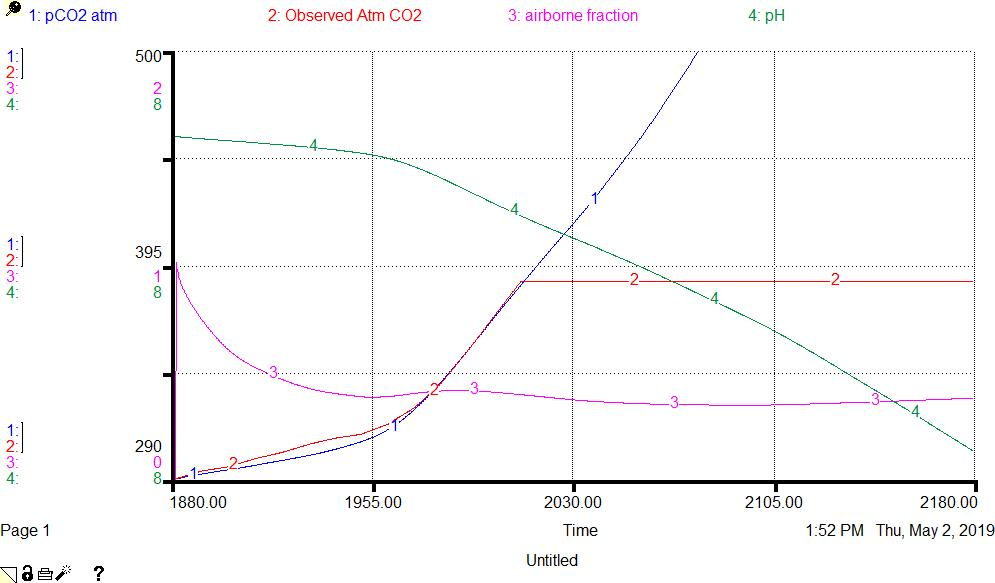
\includegraphics[width=0.9\textwidth]{./p3-1.jpg}
\end{figure}
\begin{itemize}
\item CO$_2$ levels rise at accelerating rate
\end{itemize}
}

\frame{
\frametitle{3.2. Stabilization}
\begin{figure}
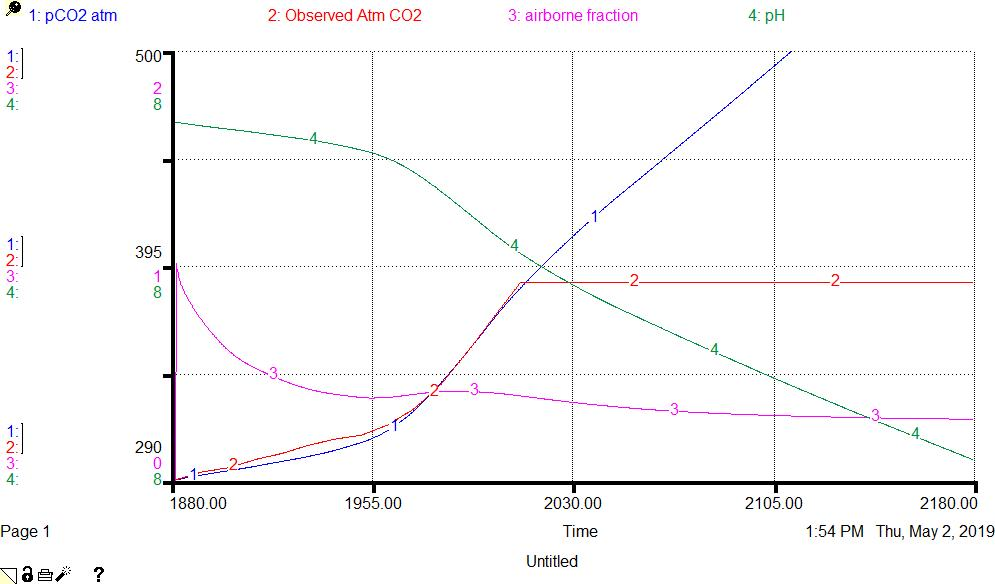
\includegraphics[width=0.9\textwidth]{./p3-2.jpg}
\end{figure}
\begin{itemize}
\item CO$_2$ continues to rise quickly; will take centuries to stabilize to new steady state
\end{itemize}
}

\frame{
\frametitle{3.3. Reduction}
\begin{figure}
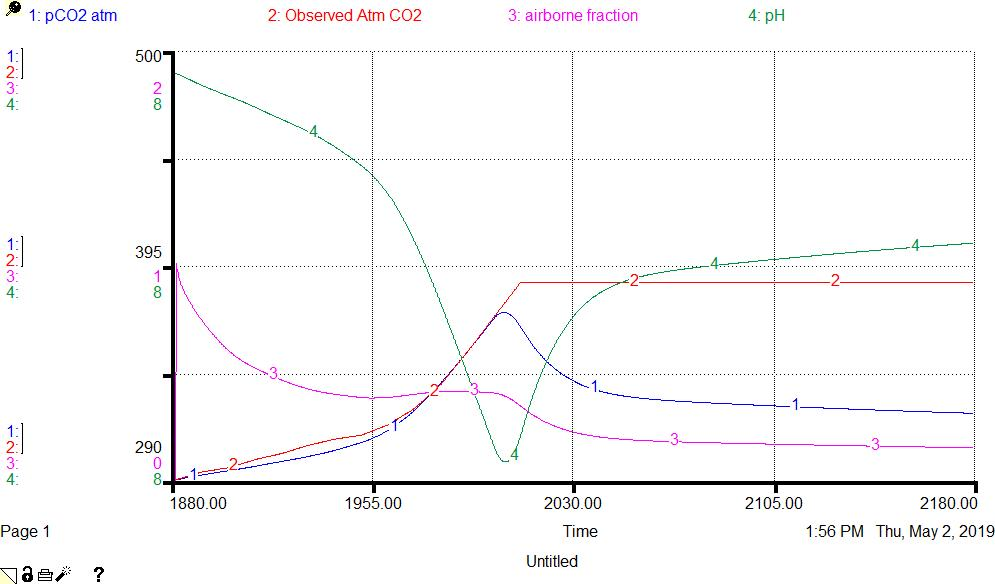
\includegraphics[width=0.9\textwidth]{./p3-3.jpg}
\end{figure}
\begin{itemize}
\item CO$_2$ nearly stabilizes after 100 years from present
\end{itemize}
}


\end{document}

\frame{
\frametitle{Key ideas}
\begin{itemize}
\item 
\end{itemize}
}

\end{document}
